% =============================================================================
% Trust and Age Bayesian Digital Twins for Network Impaired Predictive
% Maintenance in Industrial Cyber-Physical Systems
% Target: IEEE Transactions on Industrial Cyber-Physical Systems (TICPS)
% Compile: pdflatex main.tex (three times)
% =============================================================================
\documentclass[journal]{IEEEtran}
\usepackage{amsmath,amssymb,amsfonts,amsthm}
\usepackage{graphicx}
\usepackage{booktabs}
\usepackage{array}
\usepackage{float}
\usepackage{xcolor}
\usepackage[colorlinks=true,linkcolor=blue,citecolor=blue,urlcolor=blue]{hyperref}
\usepackage{orcidlink}
\usepackage{url}
\graphicspath{{figs/}}
\setlength{\textfloatsep}{5pt plus 8pt minus 1pt}
\setlength{\floatsep}{4pt plus 8pt minus 1pt}
\setlength{\dbltextfloatsep}{5pt plus 8pt minus 1pt}
\setlength{\dblfloatsep}{4pt plus 8pt minus 1pt}
\setlength{\intextsep}{5pt plus 8pt minus 1pt}
\hypersetup{
  pdftitle={Trust and Age Bayesian Digital Twins: Provable Predictive Maintenance under Industrial Network Impairments},
  pdfauthor={Yassir Ameen Al-Karawi, Hamed Al-Raweshidy},
  pdfsubject={Network-aware digital twins for predictive maintenance},
  pdfkeywords={digital twin, predictive maintenance, industrial cyber-physical systems, remaining useful life, uncertainty quantification}
}

\floatstyle{ruled}
\newfloat{algorithm}{tbp}{loa}
\floatname{algorithm}{Algorithm}

\newtheorem{theorem}{Theorem}
\newtheorem{corollary}{Corollary}
\newtheorem{proposition}{Proposition}
\newtheorem{assumption}{Assumption}
\newtheorem{remark}{Remark}

\newcommand{\E}{\mathbb{E}}
\newcommand{\Prob}{\mathbb{P}}
\newcommand{\R}{\mathbb{R}}
\newcommand{\rul}{\mathrm{RUL}}
\newcommand{\Pb}{\bar{P}}

\begin{document}

\title{Trust and Age Bayesian Digital Twins: Provable Predictive Maintenance
under Industrial Network Impairments}

\author{Yassir~Ameen~Al-Karawi\,\orcidlink{0000-0003-2959-3893},
Hamed~Al-Raweshidy\,\orcidlink{0000-0002-3702-8192}%
\thanks{Y. A. Al-Karawi is with the Department of Communications
Engineering, College of Engineering, University of Diyala, Baqubah, Diyala,
Iraq (e-mail: yassir.alkarawi@uodiyala.edu.iq).}%
\thanks{H. Al-Raweshidy is with the Wireless Networks and Communications
Centre, Department of Electronic and Electrical Engineering, College of
Engineering, Design and Physical Sciences, Brunel University London,
Uxbridge UB8 3PH, U.K. (e-mail: hamed.al-raweshidy@brunel.ac.uk).
Corresponding author: Hamed Al-Raweshidy.}}

\markboth{IEEE Transactions on Industrial Cyber-Physical Systems}%
{Al-Karawi and Al-Raweshidy: Trust and Age Bayesian Digital Twins}

\maketitle

\begin{abstract}
Predictive-maintenance digital twins often assume synchronous, equally
reliable sensor streams, although industrial packets may be delayed,
reordered, or lost. This paper introduces TABDT, a trust and age Bayesian
twin for remaining useful life (RUL) prediction under geometrically
distributed packet delays and a finite deadline. Received observations are
advanced to the current decision
time and weighted by age and sensor precision before entering a random-effects
Wiener model. For a known-drift, single-sensor scalar anchor, we derive a closed-form
steady-state variance bound, identify two RUL-error scaling regimes, and give
sufficient conditions for a unique network-dependent maintenance limit. This
guarantee is separate from TABDT's approximate delayed-data recursion. Across
4\,000 known-drift anchor paths, the bound is within 1.3\% of empirical
variance. In a separate 400-unit study, TABDT reduces RUL root-mean-square
error (RMSE) by up to 27.9\%. On all 15
XJTU-SY run-to-failure bearings, normalized RUL RMSE is 47.70 points,
compared with 52.11 for stale-as-fresh fusion and 53.02 for discard-stale
filtering. Simulated 90\% interval coverage is
93.4--95.6\%; external coverage is 76.9\%, indicating model mismatch rather
than field calibration.
\end{abstract}

\begin{IEEEkeywords}
Digital twin, predictive maintenance, industrial cyber-physical systems,
remaining useful life, Kalman filtering, age of information, uncertainty
quantification, Wiener process.
\end{IEEEkeywords}

\IEEEpeerreviewmaketitle

\section{Introduction}
\IEEEPARstart{I}{ndustrial} cyber-physical systems (ICPS) combine sensing,
communication, computation, and control. Digital twins (DTs) support
predictive maintenance (PdM) by fusing condition data with degradation models
to estimate remaining useful life (RUL)
~\cite{liu2024ticps,zhang2024ticps,tao2019}. Recent approaches often assume
synchronized, homogeneous observations
~\cite{samanazari2024ticps,kumar2025ticps}, although trustworthy deployment
depends on input quality and traceability~\cite{zhang2024ticps}.

Plant networks violate these assumptions through delayed, reordered, and lost
packets and heterogeneous sensor calibration. Treating stale data as current
biases the state estimate and understates uncertainty. Existing network-aware
DTs~\cite{alkarawi2026dt}, uncertainty guidance
~\cite{nist2023,ding2024tim}, intermittent filtering~\cite{sinopoli2004},
AoI~\cite{yates2021}, CBM codesign~\cite{ahmad2023jiot}, and robust
fusion~\cite{yang2022jiot} do not jointly connect network impairment to
first-passage prognosis. We address \emph{(G1)} a scoped network-to-RUL
certificate, \emph{(G2)} principled use of delayed measurements, and
\emph{(G3)} explicit sensor credibility.

This work makes four contributions. \emph{C1)} It couples a random-effects
Wiener model to geometrically distributed packet delay and a finite deadline.
\emph{C2)} TABDT
advances a delayed observation by the estimated degradation in transit and
weights it by $w_s(a)=\tau_s/(1+\tau_s aQ/R)$, separating sensor precision
from age uncertainty. \emph{C3)} For a known-drift, single-sensor scalar anchor,
Theorem~\ref{thm:bound}, Corollary~\ref{cor:regimes}, and
Proposition~\ref{prop:threshold} establish the variance bound, its two
RUL-error regimes, and conditional properties of the maintenance limit; these
guarantees do not extend to the approximate delayed-data recursion. \emph{C4)}
A 4\,000-path anchor experiment evaluates the bound; a separate 400-unit
common-random-number study and an XJTU-SY packet-impairment test quantify
point error and interval coverage. Code and raw results are at
\url{https://github.com/YassirALKarawi/tabdt-reproducibility} and permanently
archived as Zenodo release v19, DOI:
\href{https://doi.org/10.5281/zenodo.21861066}{10.5281/zenodo.21861066}.

\section{Related Work}\label{sec:related}

\emph{A. Digital twins for predictive maintenance:}
DT-based bearing diagnosis, cross-domain transfer, and state-space health
assessment establish the value of virtual replicas
~\cite{feng2023ticps,samanazari2024ticps,kumar2025ticps}, while the ICPS
prognostics literature centers RUL and maintenance decisions
~\cite{liu2024ticps}. Random-effects Wiener models retain inverse Gaussian
RUL, unit heterogeneity, and analytical tractability
~\cite{si2014,huang2015,zhai2017}; however, these works do not propagate
packet age and sensor credibility into the RUL posterior.

\emph{B. Imperfect networks and information aging:}
Intermittent filtering, AoI, OOSM methods, and asynchronous Bayesian filtering
address loss, freshness, delayed updates, and source-specific noise,
respectively
~\cite{sinopoli2004,yates2021,barshalom2002,barshalom2004,greiff2024cdc}.
Bursty fading also shows why mean reception probability alone is insufficient
~\cite{quevedo2013tac}. These methods do not jointly connect network quality
to first-passage RUL and asymmetric CBM costs~\cite{yang2024tr}.
Table~\ref{tab:related} positions TABDT as a link between these models, not a
new degradation law or exact OOSM replacement.

\begin{table*}[!t]
\centering
\caption{Positioning Relative to Prior Work}
\label{tab:related}
\scriptsize
\setlength{\tabcolsep}{2.7pt}
\renewcommand{\arraystretch}{0.96}
\begin{tabular}{>{\raggedright\arraybackslash}p{2.55cm}
                >{\raggedright\arraybackslash}p{3.35cm}
                >{\raggedright\arraybackslash}p{3.05cm}
                >{\raggedright\arraybackslash}p{3.55cm}
                >{\raggedright\arraybackslash}p{4.10cm}}
\toprule
Study / model & Primary prognostic role & Network treatment & Uncertainty and
sensor credibility & Decision or guarantee \\
\midrule
State-space DT health assessment~\cite{kumar2025ticps} & Synchronized virtual
replica and predictive health assessment & Data acquisition in real time is
assumed & Model and plant similarity without age-dependent sensor credibility &
Experimental condition monitoring without an anchor network-to-RUL error law \\
DT transfer diagnosis~\cite{samanazari2024ticps,feng2023ticps} &
Training data generated by a DT and fault diagnosis across domains & Packet delay,
reordering, and deadline loss are not modeled & Domain discrepancy is
learned without a provenance score $\tau_s$ or stale-packet covariance & Empirical
diagnosis without a control limit informed by the network \\
Adaptive Wiener RUL~\cite{zhai2017} & Stochastic degradation and online RUL
prediction with adaptive drift & Measurements are available to the estimator
without an explicit network & Random degradation and parameter uncertainty
with a homogeneous observation channel & Probabilistic RUL without a synchronization
certificate or PM rule \\
Intermittent Kalman filtering~\cite{sinopoli2004} & State
estimation over lossy links & Bernoulli packet arrival or loss & Error-covariance analysis for intermittent observations & Stability and covariance theory without
first-passage RUL or maintenance economics \\
AoI and OOSM methods~\cite{yates2021,barshalom2002} & Quantify information age
or update delayed tracking measurements & Explicit information age and
arrival outside sequence & State update that accounts for delay while sensor provenance is
outside scope & Timeliness or tracking correction without a DT and PdM decision chain \\
\textbf{TABDT (this work)} & \textbf{Bayesian RUL prediction and preventive
maintenance} & \textbf{Geometric age, reordering, and finite delivery
deadline} & \textbf{Joint trust and age weight $w_s(a)$ with decomposed RUL
variance $\sigma_{\rul,t}^2$} & \textbf{Closed-form $\Pb(p)$, two scaling
regimes, with $\xi^*(p)$ unique and monotone under the respective conditions
of Proposition~\ref{prop:threshold}} \\
\bottomrule
\end{tabular}
\end{table*}

\section{System Model and Problem Statement}\label{sec:model}

\subsection{Degradation Process}
Consider a fleet of nominally identical assets, using a gas-compressor bearing
as the running example. The health index (HI) $x(t)\in\R$ increases with
degradation and follows a Wiener process with a unit-specific drift,
\begin{equation}\label{eq:wiener}
\begin{aligned}
x(t)&=x_0+\mu t+\sigma_B B(t),\\
\mu&\sim\mathcal{TN}_{[\mu_{\min},\infty)}
\!\bigl(\bar\mu,\sigma_{\mu0}^{2}\bigr),\qquad \mu_{\min}>0.
\end{aligned}
\end{equation}
Here $B(t)$ is standard Brownian motion, $\sigma_B$ is the diffusion
coefficient, and $\mathcal{TN}$ is a lower-truncated normal distribution. Its
arguments denote the mean and variance of the untruncated parent normal. The
positive support gives a proper first-passage model, while $\mu$ represents
manufacturing and loading differences across units
~\cite{si2014,huang2015,zhai2017}. Failure occurs at the first crossing of the
threshold $D$. Conditional on $\mu$, the resulting time
$T_f=\inf\{t:x(t)\geq D\}$ is inverse Gaussian (IG), with mean
$(D-x_0)/\mu$ and shape $(D-x_0)^2/\sigma_B^{2}$~\cite{si2014}. Hence the
true RUL at time $t$ is $\rul_t=T_f-t$. Sampling every $\Delta t$ and setting
$x_k=x(k\Delta t)$ yields
\begin{equation}\label{eq:ss}
\mathbf{z}_{k+1}=A\,\mathbf{z}_k+\mathbf{w}_k,\quad
\mathbf{z}_k=\begin{bmatrix}x_k\\ \mu_k\end{bmatrix},\quad
A=\begin{bmatrix}1 & \Delta t\\ 0 & 1\end{bmatrix},
\end{equation}
where $\mathbf{w}_k\sim\mathcal{N}(\mathbf{0},\mathrm{diag}(Q,q_\mu))$ and
$Q=\sigma_B^{2}\Delta t$. The small random-walk variance $q_\mu$ allows the
filter to accommodate slow changes in loading without discarding the
unit-level drift model.

\subsection{Sensing and Network Model}
$S$ condition-monitoring sensors observe the HI,
\begin{equation}\label{eq:meas}
y_k^{(s)}=x_k+v_k^{(s)},\qquad
v_k^{(s)}\sim\mathcal{N}\!\bigl(0,\,R/\tau_s\bigr),\quad s=1,\dots,S.
\end{equation}
Here $R$ is nominal measurement variance and $\tau_s\in(0,1]$ is a precision
score; values below one inflate the variance. This calibration map is a TABDT
modeling choice. From held-out innovations $r_i^{(s)}$, estimate
$\widehat V_s=\max\{\epsilon_R,N_s^{-1}\sum_i[(r_i^{(s)})^2-
HP_i^-H^\top]\}$, where $H=[1\;0]$, and set
$\tau_s=\operatorname{clip}(R/\widehat V_s,\tau_{\min},1)$. Provenance may
regularize this estimate, consistent with data-quality monitoring
~\cite{nist2023} and robust channel downweighting~\cite{yang2022jiot}. Here
$\tau_s$ is fixed to isolate network effects from online trust estimation.

The packet carrying $y_k^{(s)}$ traverses the plant network with raw delay
$A_k^{(s)}$ (equivalently, its age on arrival~\cite{yates2021}),
\begin{equation}\label{eq:delay}
A_k^{(s)}\sim\mathrm{Geom}_0(p),\qquad
a_k^{(s)}=A_k^{(s)}\ \text{if }A_k^{(s)}\leq a_{\max},
\end{equation}
and is discarded if the deadline is exceeded. We refer to
$p=\Prob\{A=0\}$ as the \emph{timely synchronization probability}; the
corresponding probability of deadline loss is $(1-p)^{a_{\max}+1}$.
Analytical delays are packetwise independent, but unequal realizations can
still reorder arrivals and produce an OOSM stream
~\cite{barshalom2002,barshalom2004}.

Writing $q=1-p$ and $M=a_{\max}$, the delivered mass and its conditional
mean age follow directly from the truncated geometric series:
\begin{equation}\label{eq:agemoments}
\begin{aligned}
P_{\mathrm{del}}(p)&=\sum_{a=0}^{M}pq^a=1-q^{M+1},\\
\bar a_{\mathrm{del}}(p)&=\E[A\mid A\leq M]
=\frac{q[1-(M+1)q^M+Mq^{M+1}]}{p(1-q^{M+1})}.
\end{aligned}
\end{equation}
Thus $1-P_{\mathrm{del}}$ measures missing information, whereas
$\bar a_{\mathrm{del}}$ measures the staleness of retained packets.

\subsection{Problem Statement}
At step $k$, the twin must use only arrived packets to report
$\widehat{\rul}_k$, a nominal $(1-\alpha)$ approximate prediction interval,
and a preventive-maintenance (PM) trigger. We seek an accuracy guarantee for
a tractable anchor model as a function of $p$ and a fusion rule that does not
overstate the information in stale or low-credibility observations.
Table~\ref{tab:notation} summarizes the notation.

\begin{table}[!t]
\centering
\caption{Principal Notation}
\label{tab:notation}
\begin{tabular}{ll}
\toprule
Symbol & Meaning \\
\midrule
$x_k$, $D$ & health index at step $k$, failure threshold \\
$\mu$, $\bar\mu$, $\sigma_{\mu0}$ & unit drift, parent-normal mean and SD \\
$\sigma_B$, $Q$ & diffusion coefficient and process variance $\sigma_B^2\Delta t$ \\
$y_k^{(s)}$, $R$, $\tau_s$ & measurement, nominal variance, sensor precision \\
$a_k^{(s)}$, $p$, $q$, $a_{\max}$ & packet age, timely probability, $1-p$, deadline \\
$w_s(a)$, $\eta^{*}$ & trust and age weight with $\eta^{*}=Q/R$ \\
$P_{\mathrm{del}}$ & probability of delivery before the deadline \\
$\hat{\mathbf z}_k$, $P_k$ & state estimate and error covariance \\
$\Pb(p)$ & steady-state variance bound (Thm.~\ref{thm:bound}) \\
$\xi$, $\xi^{*}$ & PM control limit and its optimum (Prop.~\ref{prop:threshold}) \\
$c_p$, $c_f$ & preventive / failure replacement cost \\
\bottomrule
\end{tabular}
\end{table}

\section{The TABDT Framework}\label{sec:framework}

The architecture in Fig.~\ref{fig:arch} follows the path of a measurement
from the physical asset to the maintenance decision. Its three central design
choices---age compensation, joint trust--age weighting, and a
network-informed PM limit---correspond to gaps G1--G3 identified above.

\begin{figure*}[!t]
\centering
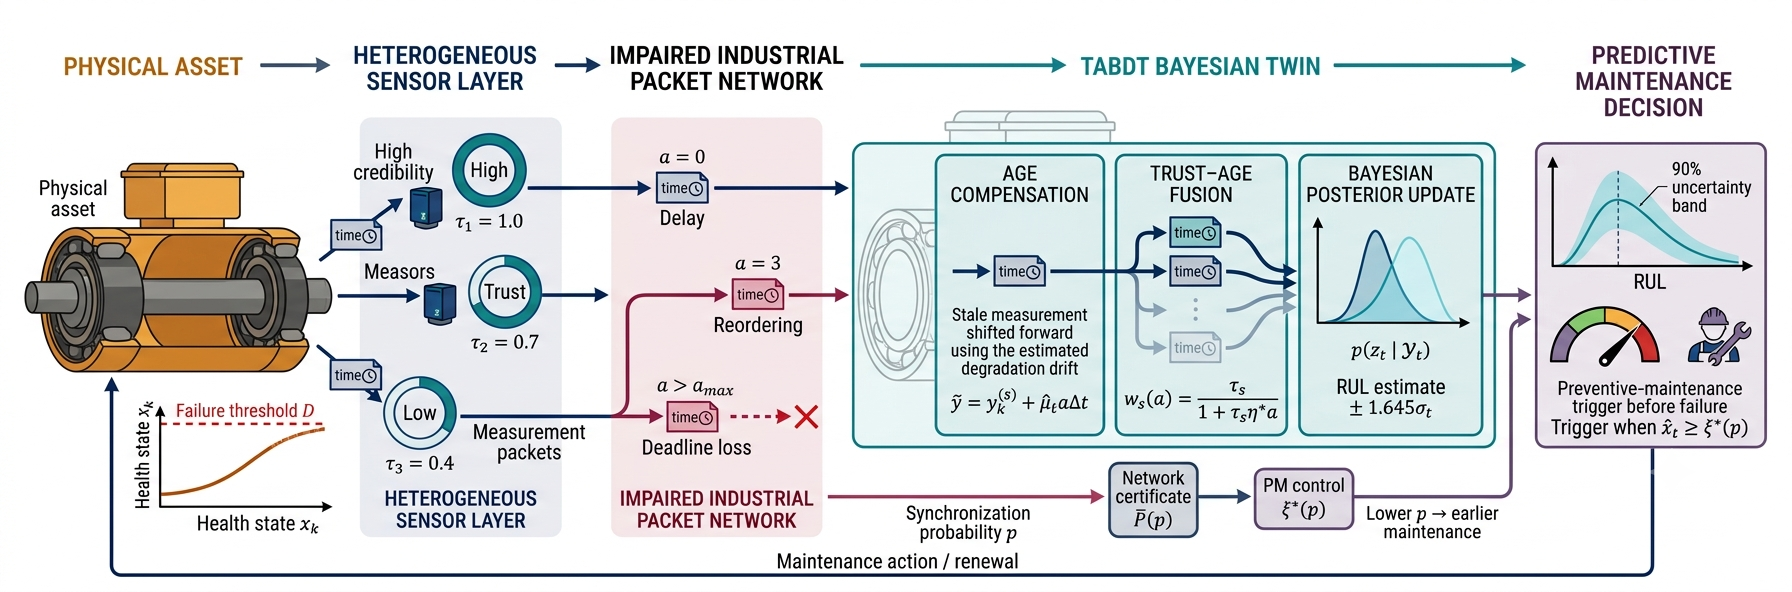
\includegraphics[width=0.90\textwidth]{fig1_architecture.png}
\caption{End-to-end TABDT architecture. Timestamped sensor observations undergo
delay, reordering, and deadline loss. Age compensation, trust--age fusion, and
Bayesian updating yield state and RUL posteriors. The certificate $\Pb(p)$
provides the scale for the surrogate preventive-maintenance limit
$\xi^*(p)$.}
\label{fig:arch}
\end{figure*}

\subsection{Age Compensation with Trust and Age Weighting}
A packet $(y_k^{(s)},k,s)$ arriving at step $t$ with age $a=t-k$ measures
the past state $x_{k}$ rather than the current state. The two are related by
$x_t=x_k+\mu a\Delta t+\nu_{k:t}$, where
$\nu_{k:t}=\sum_{j=k+1}^{t}\varepsilon_j\sim\mathcal N(0,aQ)$. After
shifting the packet by the estimated drift, its residual with respect to the
current state is
\begin{equation}\label{eq:residual}
\tilde y-H\mathbf z_t
=v_k^{(s)}-\nu_{k:t}+a\Delta t(\hat\mu_t-\mu),
\qquad H=[1\;0].
\end{equation}
An exact OOSM retrodiction would retain both state--measurement covariance and
the dependence between delayed packets~\cite{barshalom2002,barshalom2004}.
TABDT uses a cheaper forward correction: it holds the current drift fixed
over the packet age and neglects correlations induced by shared process
noise. Under this first-order conditional-independence approximation,
\eqref{eq:residual} has marginal variance
\begin{equation}\label{eq:reff}
R_{s,a}^{\mathrm{eff}}
=\frac{R}{\tau_s}+aQ+(a\Delta t)^2[P_t]_{\mu\mu}.
\end{equation}
The estimator therefore advances the observation by the degradation missed
in transit and assigns the retained marginal uncertainty to its likelihood:
\begin{align}
\tilde{y} &= y_k^{(s)}+\hat{\mu}_t\,a\Delta t, \label{eq:agecomp}\\
\tilde{R} &= \frac{R}{w}\;+\;(a\Delta t)^{2}\,[P_t]_{\mu\mu},
\qquad w=w_s(a)=\frac{\tau_s}{1+\tau_s\eta a}. \label{eq:weight}
\end{align}
Using \eqref{eq:agecomp} and \eqref{eq:weight} sequentially does not recover
the exact delayed-data posterior. This distinction is kept explicit, and the
sensitivity, coverage, and exact-reprocessing experiments later quantify its
practical consequence. For a fresh packet, $\tau_s$ controls the sensor
variance; for a delayed packet, $a$ discounts information further. Since
$R/w_s(a)=R/\tau_s+\eta aR$, choosing
\begin{equation}\label{eq:etastar}
\eta^{*}=Q/R
\end{equation}
makes $R/w_s(a)=R/\tau_s+aQ$: the nominal sensor contribution plus the Wiener
variance accumulated during transit. The age rate is consequently the ratio
of process to measurement variance, and it has the expected monotonicity
\begin{equation}\label{eq:weightderivatives}
\frac{\partial w_s}{\partial a}
=-\frac{\tau_s^2\eta}{(1+\tau_s\eta a)^2}<0,
\qquad
\frac{\partial w_s}{\partial\tau_s}
=\frac{1}{(1+\tau_s\eta a)^2}>0.
\end{equation}
Section~\ref{sec:results} varies this ratio over four orders of magnitude.
The remaining term in \eqref{eq:weight} accounts for uncertainty in the drift
estimate; without it, an old packet would receive excessive weight precisely
when the forward shift is least certain.

Finally, a delivered packet is fused once and only once. Reusing the last
stored value in later updates would count the same observation repeatedly.

\subsection{Bayesian Recursion}
Equations~\eqref{eq:agecomp} and \eqref{eq:weight} define the measurement
updates in a standard sequential Kalman recursion for \eqref{eq:ss}. Each step
applies a time update followed by one scalar update per newly arrived packet,
using $H=[1\;\,0]$, $\tilde y$, and $\tilde R$. Algorithm~\ref{alg:tabdt}
specifies packet order and single use. The prior $\hat\mu_0=\bar\mu$, with
variance $\sigma_{\mu0}^{2}$, uses the parent-normal moments as a Gaussian
approximation to the truncated prior; state augmentation learns the unit
drift~\cite{zhai2017}.

\begin{algorithm}[!t]
\caption{Trust and age Bayesian recursion at time $t$}
\label{alg:tabdt}
\scriptsize
\setlength{\tabcolsep}{2pt}
\begin{tabular}{@{}r@{\ }p{0.89\columnwidth}@{}}
\toprule
\multicolumn{2}{@{}>{\raggedright\arraybackslash}p{0.98\columnwidth}@{}}{\textbf{Require:} posterior
$(\hat{\mathbf z}_{t-1},P_{t-1})$, unused packets $\mathcal A_t$,
$Q,q_\mu,R,\{\tau_s\},\eta^{*},D,\Delta t,\sigma_B,\alpha,
\epsilon_x,\epsilon_\mu,\xi^*(p)$}\\
\multicolumn{2}{@{}>{\raggedright\arraybackslash}p{0.98\columnwidth}@{}}{\textbf{Invariant:} each packet is fused once, in
nondecreasing age $a=t-k$ (newest first).}\\
\midrule
1: & \textbf{Predict:}
$\hat{\mathbf z}\leftarrow A\hat{\mathbf z}_{t-1}$,
$P\leftarrow AP_{t-1}A^\top+\mathrm{diag}(Q,q_\mu)$.\\
2: & Sort $\mathcal A_t$ by $(a,s)$. \textbf{For each}
$(y_k^{(s)},k,s)\in\mathcal A_t$ \textbf{do}\\
3: & \quad $a\leftarrow t-k$ and
$w\leftarrow\tau_s/(1+\tau_s\eta^{*}a)$.\\
4: & \quad Let $\hat\mu=[\hat{\mathbf z}]_\mu$ and
$P_{\mu\mu}=[P]_{\mu\mu}$; set
$\tilde y\leftarrow y_k^{(s)}+\hat\mu a\Delta t$ and
$\tilde R\leftarrow R/w+(a\Delta t)^2P_{\mu\mu}$.\\
5: & \quad $K\leftarrow PH^\top(HPH^\top+\tilde R)^{-1}$ and
$e\leftarrow\tilde y-H\hat{\mathbf z}$.\\
6: & \quad $\hat{\mathbf z}\leftarrow\hat{\mathbf z}+Ke$,
$J\leftarrow I-KH$, and
$P\leftarrow JPJ^\top+K\tilde R K^\top$.\\
7: & \textbf{End for}. Symmetrize $P\leftarrow(P+P^\top)/2$, then set
$\hat{\mathbf z}_t\leftarrow\hat{\mathbf z}$ and $P_t\leftarrow P$.\\
8: & Evaluate \eqref{eq:rulmean} through \eqref{eq:rulvar}. Set
$u_t\leftarrow\mathbf 1\{\hat x_t\geq\xi^*(p)\}$.\\
\midrule
\multicolumn{2}{@{}>{\raggedright\arraybackslash}p{0.98\columnwidth}@{}}{\textbf{Ensure:} $\hat{\mathbf z}_t,P_t$,
$\widehat{\rul}_t\pm z_{1-\alpha/2}\sigma_{\rul,t}$, and PM flag $u_t$.}\\
\bottomrule
\end{tabular}
\end{algorithm}

\subsection{RUL Posterior}
Given the posterior mean
$\hat{\mathbf z}_t=[\hat x_t,\hat\mu_t]^{\top}$ and covariance $P_t$, define
$m_t=\max(D-\hat x_t,\epsilon_x)$ and
$\hat\mu_t^+=\max(\hat\mu_t,\epsilon_\mu)$. The forecast holds the drift fixed
beyond $t$. This is exact when $q_\mu=0$ and is a local approximation for the
slow random walk in \eqref{eq:ss}. Under that approximation, the first-passage RUL
$L_t=T_f-t$ has the inverse Gaussian density
\begin{equation}\label{eq:igdensity}
f_{L_t\mid x_t,\mu}(\ell)
=\frac{D-x_t}{\sqrt{2\pi\sigma_B^2\ell^3}}
\exp\!\left[-\frac{(D-x_t-\mu\ell)^2}
{2\sigma_B^2\ell}\right],\quad \ell>0.
\end{equation}
The conditional mean and variance of \eqref{eq:igdensity} are
$(D-x_t)/\mu$ and $(D-x_t)\sigma_B^2/\mu^3$, respectively. Evaluating the
mean at the posterior estimates gives the point predictor
\begin{equation}\label{eq:rulmean}
\widehat{\rul}_t=\frac{m_t}{\hat\mu_t^+}.
\end{equation}
For $g(x,\mu)=(D-x)/\mu$, when $D-\hat x_t>\epsilon_x$ and
$\hat\mu_t>\epsilon_\mu$ the safeguards are inactive and the gradient at the
posterior mean is
\begin{equation}\label{eq:rulgradient}
\nabla g_t=
\begin{bmatrix}-(\hat\mu_t^+)^{-1}&
-m_t(\hat\mu_t^+)^{-2}\end{bmatrix}^{\!\top}.
\end{equation}
If either safeguard is active, \eqref{eq:rulgradient} is instead used as a
stabilized plug-in expression.
Applying the law of total variance and the first-order delta method gives
\begin{equation}\label{eq:totalvariance}
\operatorname{Var}(L_t\mid\mathcal Y_t)
\approx \E[\operatorname{Var}(L_t\mid\mathbf z_t)\mid\mathcal Y_t]
+\nabla g_t^\top P_t\nabla g_t.
\end{equation}
Substituting \eqref{eq:rulgradient} into \eqref{eq:totalvariance} separates
the aleatoric first-passage part and the epistemic
state-estimation part~\cite{si2014}:
\begin{equation}\label{eq:rulvar}
\sigma_{\rul,t}^{2}
\approx\underbrace{\frac{m_t\sigma_B^{2}}{(\hat\mu_t^+)^{3}}}_{\text{aleatoric (IG)}}
+\underbrace{\frac{[P_t]_{xx}}{(\hat\mu_t^+)^{2}}
+\frac{m_t^2[P_t]_{\mu\mu}}{(\hat\mu_t^+)^{4}}
+\frac{2m_t[P_t]_{x\mu}}{(\hat\mu_t^+)^{3}}}_{\text{epistemic (delta method)}} .
\end{equation}
The nominal interval is
$\widehat{\rul}_t\pm z_{1-\alpha/2}\sigma_{\rul,t}$. It should not be
interpreted as an exact Bayesian credible interval: \eqref{eq:rulvar} inserts
the expected aleatoric component and neglects higher posterior moments. Its
coverage must therefore be established empirically~\cite{ding2024tim}. The
delta expansion does, however, retain the state--drift covariance. The result
in the next section bounds the $[P_t]_{xx}$ contribution only for the stated
anchor filter; it is not a bound on Algorithm~\ref{alg:tabdt} with unknown
drift and approximate OOSM updates.

\section{Theoretical Guarantees}\label{sec:theory}

\subsection{A Closed-Form Variance Certificate}
For analytical tractability, consider a unit-trust, known-drift,
single-sensor scalar anchor that accepts fresh packets and omits delayed ones.
This reference model is separate from the approximate OOSM recursion in
Algorithm~\ref{alg:tabdt}. Let $P_k$ be its one-step-ahead prior variance.
Because a fresh measurement is available with probability $p$ at each step
~\cite{sinopoli2004}, $P_k$ obeys
\begin{equation}\label{eq:riccati}
P_{k+1}=P_k+Q-\gamma_k\,\frac{P_k^{2}}{P_k+R},
\qquad \gamma_k\sim\mathrm{Bern}(p).
\end{equation}

\begin{theorem}[Steady-state variance bound]\label{thm:bound}
For the scalar health submodel induced by \eqref{eq:ss} under known drift,
suppose $\gamma_k$ in \eqref{eq:riccati} is independent of $P_k$. Then, for
any $p\in(0,1]$,
\begin{equation}\label{eq:bound}
\limsup_{k\to\infty}\E[P_k]\;\leq\;
\Pb(p)\;=\;\frac{Q+\sqrt{Q^{2}+4pQR}}{2p}.
\end{equation}
\end{theorem}

\begin{proof}
Write $g(P)=P^{2}/(P+R)$. Since $g''(P)=2R^{2}/(P+R)^{3}>0$, $g$ is convex
on $[0,\infty)$, and Jensen's inequality gives
$\E[g(P_k)]\geq g(\E[P_k])$. Taking expectations of \eqref{eq:riccati},
\[
\E[P_{k+1}]=\E[P_k]+Q-p\,\E[g(P_k)]\;\leq\;f\bigl(\E[P_k]\bigr),
\]
with $f(u)=u+Q-p\,g(u)$. Because
$g'(u)=(u^{2}+2uR)/(u+R)^{2}\in[0,1)$, the derivative $f'(u)\in(1-p,1]$.
Hence $f$ is nondecreasing, and the comparison sequence $u_{k+1}=f(u_k)$,
$u_0=\E[P_0]$, dominates $\E[P_k]$ for all $k$. The fixed points of $f$
solve $Q=p\,g(u)$, i.e., $p u^{2}-Qu-QR=0$, whose unique positive root is
$\Pb(p)$ in \eqref{eq:bound}. Since $f(u)-u=Q-p\,g(u)$ is positive below
$\Pb(p)$ and negative above it, and $f$ is monotone, $u_k\to\Pb(p)$ from
any initialization, which yields the claim.
\end{proof}

Implicit differentiation of $p\Pb^2=Q(\Pb+R)$ gives
\begin{equation}\label{eq:boundmonotonicity}
\frac{d\Pb}{dp}=-\frac{\Pb^2}{2p\Pb-Q}
=-\frac{\Pb^2}{\sqrt{Q^2+4pQR}}<0.
\end{equation}
Equation~\eqref{eq:boundmonotonicity} shows that the variance bound increases
strictly as the synchronization probability decreases.

\begin{corollary}[Two network scaling regimes]\label{cor:regimes}
For the known-drift anchor filter, let $\delta=Q/(pR)$. If
$\delta\to0$ (equivalently, $p\gg Q/R$), then
\begin{equation}\label{eq:quarter}
\begin{aligned}
\Pb(p)&=\sqrt{\frac{QR}{p}}\,[1+O(\!\sqrt\delta)],\\
\sigma_{\rul}^{\mathrm{epi}}&\lesssim
\frac{(QR)^{1/4}}{\mu}p^{-1/4}[1+O(\!\sqrt\delta)].
\end{aligned}
\end{equation}
In the extreme-loss limit $pR/Q\to0$,
\begin{equation}\label{eq:halfpow}
\Pb(p)=\frac{Q}{p}+R+O\!\left(\frac{pR^2}{Q}\right),\qquad
\sigma_{\rul}^{\mathrm{epi}}\lesssim\frac{\sqrt Q}{\mu}p^{-1/2}.
\end{equation}
\end{corollary}

For these parameters, $Q/R=9\times10^{-4}$ and $p\geq0.02$, so
$\delta\leq0.045$ and \eqref{eq:quarter} applies. Halving $p$ then increases
the leading epistemic RUL scale by $2^{1/4}-1\approx18.9\%$. In contrast,
\eqref{eq:halfpow} gives the extreme-loss RUL-error exponent $-1/2$. Because
TABDT retains delayed packets, the bound is used only as a network-dependent
scale, not a guarantee for the full recursion.

\subsection{Maintenance Threshold Informed by the Network}
We next use the certificate to parameterize a preventive-maintenance cost
model. Under the classical control-limit policy~\cite{yang2024tr}, the asset is
replaced preventively (cost $c_p$) when the \emph{estimate} $\hat x$ crosses
$\xi<D$. An undetected crossing of $D$ before the trigger costs
$c_f>c_p$. Let $e_k=x_k-\hat x_k$ denote the zero-mean anchor-filter error.
An unnoticed failure requires $e_k$ to exceed the safety margin $m=D-\xi$.
Theorem~\ref{thm:bound} gives the distribution-free Cantelli bound
\begin{equation}\label{eq:cantelli}
\limsup_{k\to\infty}\Prob\{e_k\geq m\}
\leq \frac{\Pb(p)}{\Pb(p)+m^2},\qquad m>0.
\end{equation}
Variance alone does not imply a Gaussian tail. We therefore introduce the
following smooth surrogate, whose accuracy can be checked by simulation:
\begin{equation}\label{eq:cost}
C_G(\xi,p)\;\triangleq\;\Bigl[c_p+(c_f-c_p)\,
\bar\Phi\!\Bigl(\tfrac{D-\xi}{\sqrt{\Pb(p)}}\Bigr)\Bigr]\,
\frac{\mu}{\xi},
\end{equation}
where $\bar\Phi$ and $\phi$ denote the standard normal tail and density. The
bracketed factor approximates expected replacement cost, while $\mu/\xi$
approximates the renewal rate. Unlike the Cantelli result in
\eqref{eq:cantelli}, $C_G$ is a design surrogate rather than a probabilistic
upper bound.

\begin{proposition}[Unique control limit and network monotonicity]\label{prop:threshold}
Let $s=\sqrt{\Pb(p)}$ and $d=c_f-c_p>0$. If
\begin{equation}\label{eq:interiorcondition}
\frac{Dd}{s\sqrt{2\pi}}>\frac{c_f+c_p}{2},
\end{equation}
the surrogate \eqref{eq:cost} has a unique interior minimizer
$\xi^{*}\in(0,D)$ characterized by
\begin{equation}\label{eq:foc}
(c_f-c_p)\,\frac{\xi^{*}}{\sqrt{\Pb(p)}}\,
\phi\!\Bigl(\tfrac{D-\xi^{*}}{\sqrt{\Pb(p)}}\Bigr)
= c_p+(c_f-c_p)\,\bar\Phi\!\Bigl(\tfrac{D-\xi^{*}}{\sqrt{\Pb(p)}}\Bigr).
\end{equation}
Let $r^*=(D-\xi^*)/s$. Wherever $(r^*)^2\xi^*>D$, the safety margin
$D-\xi^*$ is strictly increasing in $s$ and hence nonincreasing in $p$.
\end{proposition}

\begin{proof}
Write $h(\xi)=c_p+d\bar\Phi((D-\xi)/s)$, so $C_G'(\xi,p)$ has the sign of
$F(\xi)=\xi h'(\xi)-h(\xi)$. Here $F(0)<0$, condition
\eqref{eq:interiorcondition} is exactly $F(D)>0$, and
$F'(\xi)=\xi h''(\xi)>0$ for $0<\xi<D$. Hence the root is unique and gives
\eqref{eq:foc}. Implicit differentiation of \eqref{eq:foc} gives
$\mathrm d(D-\xi^*)/\mathrm ds=r^*-D/(r^*\xi^*)$, which is positive under
the stated condition. Finally, $s$ decreases with $p$ by \eqref{eq:bound}.
\end{proof}

The surrogate combines a Gaussian tail with a first-order renewal scale and
does not model diffusion overshoot near $D$; both approximations are examined
in Section~\ref{sec:results}. Let
$F_p(\xi)=\xi h'(\xi)-h(\xi)$ be the stationary-point residual from the proof
of Proposition~\ref{prop:threshold}. Under
\eqref{eq:interiorcondition}, $F_p$ is strictly increasing, so a bracketed root
solve is preferable to an unconstrained optimizer. Algorithm~\ref{alg:threshold}
implements this calculation and, under the stated condition, returns the
unique stationary point. If the condition fails and $F_p(D)\leq0$, the
surrogate decreases throughout $(0,D)$; its strict-domain infimum occurs as
$\xi\uparrow D$, and the implementation returns the $\epsilon$-interior
approximation $D-\epsilon$.

\begin{algorithm}[!t]
\caption{PM threshold informed by the network}
\label{alg:threshold}
\scriptsize
\setlength{\tabcolsep}{2pt}
\begin{tabular}{@{}r@{\ }p{0.875\columnwidth}@{}}
\toprule
\multicolumn{2}{@{}>{\raggedright\arraybackslash}p{0.98\columnwidth}@{}}{\textbf{Require:} $p,Q,R,D,\mu,c_p,c_f$ and
root tolerance $0<\epsilon<D$.}\\
\midrule
1: & $\Pb\leftarrow(Q+\sqrt{Q^2+4pQR})/(2p)$,
$s\leftarrow\sqrt{\Pb}$, and $d\leftarrow c_f-c_p$.\\
2: & $h(\xi)\leftarrow c_p+d\bar\Phi((D-\xi)/s)$ and
$F_p(\xi)\leftarrow\xi d\phi((D-\xi)/s)/s-h(\xi)$.\\
3: & \textbf{if} $F_p(D)\leq0$ \textbf{then} set $\xi^*\leftarrow D-\epsilon$
and evaluate $C_G(\xi^*,p)$; \textbf{return}.\\
4: & \textbf{else} solve $F_p(\xi)=0$ on $(0,D)$ by a safeguarded bracketed
method (bisection/Brent) until the bracket width is at most $\epsilon$.\\
5: & Set $\xi^*$ to the bracketed root. Evaluate $C_G(\xi^*,p)$ from
\eqref{eq:cost}.\\
\midrule
\multicolumn{2}{@{}>{\raggedright\arraybackslash}p{0.98\columnwidth}@{}}{\textbf{Ensure:} unique interior $\xi^*(p)$ when
\eqref{eq:interiorcondition} holds; otherwise, an $\epsilon$-interior
approximation to the boundary infimum.}\\
\bottomrule
\end{tabular}
\end{algorithm}

\subsection{Computational Complexity}
Let $m_t=|\mathcal A_t|$. One step of Algorithm~\ref{alg:tabdt} costs
$O(n^3+m_tn^2+m_t\log m_t)$ operations and $O(n^2+m_t)$ memory. In steady
state $\E[m_t]=SP_{\mathrm{del}}\leq S$, whereas the deadline gives
$m_t\leq S(a_{\max}+1)$. For the fixed state dimension $n=2$, the expected
per-step complexity is therefore $O(Sn^2)$, although a deadline-sized burst
can be more expensive. Algorithm~\ref{alg:threshold} requires
$O(\log(D/\epsilon))$ root iterations. These operation counts exclude
platform-dependent latency and energy consumption, which require
implementation-level profiling.

\section{Numerical Study}\label{sec:results}

\subsection{Simulation Setup and Model Verification}
Table~\ref{tab:params} specifies a bearing with $\bar\mu=0.02$ HI/h, nominal
mean life 500 h, and three unequal-precision sensors. The range $p=0.02$ to 1
spans a 13.0\% deadline-loss case ($a_{\max}=100$) to ideal delivery.
Simulator verification over 20\,000 fixed-drift paths gave failure-time mean
and standard deviation 501.3 h and 33.6 h, versus IG values 500.0 h and
33.5 h.

\begin{table}[!t]
\centering
\caption{Simulation Configuration}
\label{tab:params}
\begin{tabular}{llll}
\toprule
Parameter & Value & Parameter & Value \\
\midrule
$\Delta t$ & 1 h & $D$ & 10 HI \\
$\bar\mu$ & 0.02 HI/h & $\sigma_{\mu0}$ & 0.004 HI/h \\
$\mu_{\min}$ & 0.01 HI/h & $P_0$ & $\mathrm{diag}(0.25,\sigma_{\mu0}^2)$ \\
$\sigma_B$ & 0.03 HI/$\sqrt{\mathrm{h}}$ & $Q$ & $9\times10^{-4}$ \\
$R$ & 1.0 & $(\tau_1,\tau_2,\tau_3)$ & $(1.0,\,0.7,\,0.4)$ \\
$q_\mu$ & $10^{-7}$ & $\eta^{*}=Q/R$ & $9\times10^{-4}$ \\
$a_{\max}$ & 100 steps & $(c_p,c_f)$ & $(1,\,10)$ \\
Monte Carlo units & 400 & eval.\ window & $[0.2,\,0.9]\,T_f$ \\
\bottomrule
\end{tabular}
\end{table}

\subsection{Baselines and Metrics}\label{sec:metrics}
All four estimators use the same degradation paths, measurement noise, and
packet realizations. B1 uses only the degradation model and parent-normal
reference drift;
B2 applies every delivered packet as current; B3 accepts only on-time packets
~\cite{sinopoli2004}; and TABDT follows Algorithm~\ref{alg:tabdt}. RUL RMSE
and nominal 90\% prediction-interval coverage (PICP) are evaluated over
20--90\% of each life. Common paths, Gaussian draws, and inverse-CDF delay
uniforms are reused across $p$. Plots show descriptive bars equal to
$\pm1.96$ standard errors from unweighted unit-level metrics; because the
centers are pooled point-time metrics, these are not confidence intervals for
the plotted estimands. For
$\mathcal I=\{(n,k):0.2T_f^{(n)}\leq k\Delta t\leq0.9T_f^{(n)}\}$, the metrics
are
\begin{equation}\label{eq:metrics}
\begin{aligned}
e_{n,k}&=\widehat{\rul}_{n,k}-\rul_{n,k},\\
\mathrm{RMSE}_{\rul}
&=\left[|\mathcal I|^{-1}\!\sum_{(n,k)\in\mathcal I}e_{n,k}^{2}\right]^{1/2},\\
\mathrm{PICP}_{0.9}
&=|\mathcal I|^{-1}\!\sum_{(n,k)\in\mathcal I}
\mathbf 1\!\left\{|e_{n,k}|\leq1.645\,\sigma_{\rul,n,k}\right\}.
\end{aligned}
\end{equation}
\subsection{Results}

\emph{1) Representative trajectory:}
Fig.~\ref{fig:traj} shows a unit at $p=0.4$. Timely packets arrive
irregularly; prediction and subsequent updates progressively reflect its
drift in the state estimate and the 90\% RUL limits from \eqref{eq:rulvar}.

\begin{figure}[!t]
\centering
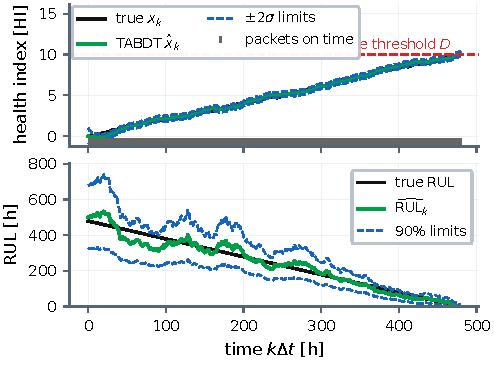
\includegraphics[width=\columnwidth]{fig2_trajectories}
\caption{One realization at $p=0.4$. Top: true and estimated health index
with paired $\pm2\sigma$ limits, failure threshold $D$, and packets arriving
on time (rug marks). Bottom: true RUL against the TABDT estimate
\eqref{eq:rulmean} with paired 90\% limits from \eqref{eq:rulvar}.}
\label{fig:traj}
\end{figure}

\emph{2) RUL accuracy under network degradation:}
Figure~\ref{fig:rmse} and Table~\ref{tab:headline} give the main comparison.
At $p=1$, the measurement-based estimators coincide at 54.0 h; B1 remains at
121.2 h because it never learns unit drift. At $p=0.02$, TABDT records 64.3 h
versus 75.3 h for B3 and 89.1 h for B2, reductions of 14.7\% and 27.9\%.
At $p=0.05$, its 58.3 h RMSE is 9.2\% and 10.7\% lower, respectively.
TABDT remains within 54.0--58.3 h for $p\geq0.05$, so a twentyfold decrease
from $p=1$ to 0.05 adds 4.3 h in this experiment.

At $p=0.02$, delivered packets have mean age 33.9 steps; treating them as
current omits about
$\bar\mu\,\E[a\mid a\leq a_{\max}]\Delta t=0.68$ HI. TABDT restores this
drift and includes $aQ+(a\Delta t)^2P_{\mu\mu}$ in the variance, whereas B3
avoids bias by rejecting delayed information.

\begin{figure}[!t]
\centering
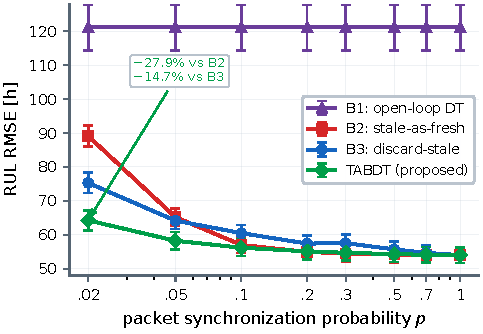
\includegraphics[width=\columnwidth]{fig3_rmse_vs_p}
\caption{RUL RMSE against timely synchronization probability $p$ on a log
scale. Bars are the descriptive quantities in Section~\ref{sec:metrics};
measurement-based methods coincide at $p=1$.}
\label{fig:rmse}
\end{figure}

\begin{table}[!t]
\centering
\caption{Headline Comparison at Three Network Conditions}
\label{tab:headline}
\setlength{\tabcolsep}{3.6pt}
\begin{tabular}{lcccccc}
\toprule
& \multicolumn{2}{c}{$p=0.02$} & \multicolumn{2}{c}{$p=0.05$}
& \multicolumn{2}{c}{$p=0.20$} \\
\cmidrule(lr){2-3}\cmidrule(lr){4-5}\cmidrule(lr){6-7}
Method & RMSE & PICP & RMSE & PICP & RMSE & PICP \\
& [h] & [\%] & [h] & [\%] & [h] & [\%] \\
\midrule
B1 open-loop      & 121.2 & 95.0 & 121.2 & 95.0 & 121.2 & 95.0 \\
B2 stale-as-fresh & 89.1 & 91.5 & 65.2 & 97.0 & \textbf{55.0} & 96.4 \\
B3 discard-stale  & 75.3 & 95.7 & 64.2 & 95.8 & 57.4 & 95.9 \\
TABDT (proposed) & \textbf{64.3} & 93.4 & \textbf{58.3} & 94.5
                  & 55.1 & 95.2 \\
\bottomrule
\end{tabular}
\end{table}

\emph{3) Prediction-interval coverage:}
Calibration is distinct from point accuracy~\cite{ding2024tim}.
Figure~\ref{fig:picp} shows conservative synthetic intervals: TABDT covers
93.4--95.6\%, B3 95.5--95.9\%, and B2 91.5\% at $p=0.02$ but 95.6--97.2\%
elsewhere. Thus the RMSE gain alone does not establish calibration.

\begin{figure}[!t]
\centering
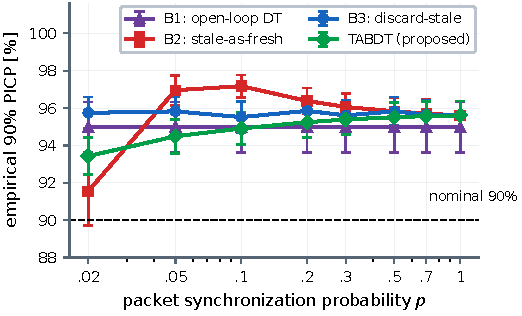
\includegraphics[width=\columnwidth]{fig4_picp}
\caption{Empirical coverage $\mathrm{PICP}_{0.9}$ on a log abscissa. Bars are
defined in Section~\ref{sec:metrics}; the dashed line is the nominal 90\%
target. TABDT covers 93.4--95.6\%.}
\label{fig:picp}
\end{figure}

\emph{4) Tightness of the analytical bound:}
Across 4\,000 anchor paths in Fig.~\ref{fig:thm},
$\Pb(p)/\E[P]$ ranges from 1.000 at $p=1$ to 1.013 at $p=0.05$. The
$\sqrt{QR/p}$ curve has the moderate-loss variance slope $-1/2$; below
$p\approx Q/R$, \eqref{eq:halfpow} instead gives the $p\to0$ slope $-1$.
Proposition~\ref{prop:threshold} uses the closed-form bound, not this
moderate-regime approximation.

\begin{figure}[!t]
\centering
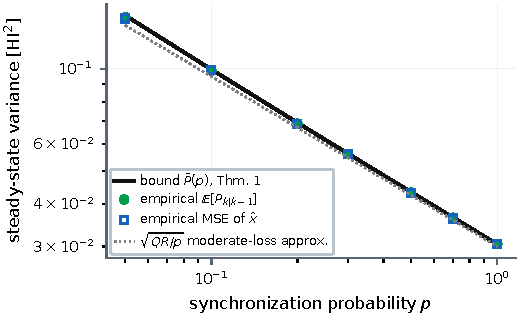
\includegraphics[width=\columnwidth]{fig5_theorem1}
\caption{Validation of Theorem~\ref{thm:bound}. The closed-form bound
$\Pb(p)$ exceeds the empirical prior variance and MSE at every evaluated
$p$, with at most 1.3\% slack over this range, and follows the
$\sqrt{QR/p}$ moderate-loss approximation.}
\label{fig:thm}
\end{figure}

\emph{5) Sensitivity and external age-compensation test:}
The prespecified $\eta/\eta^*$ sweep changes RMSE by at most 6.5\%; at
$p=0.05$, ratios 1 and 100 give 54.7 and 51.2 h. This tests robustness, not
empirical optimality of $\eta^*$.

A single-channel XJTU-SY test uses all 15 bearing lives under three operating
conditions (9\,216 one-minute records; 32\,768 samples per record)
~\cite{wang2020xjtu}. Although two channels are recorded, the proxy uses only
horizontal-vibration peak amplitude $h$:
$\operatorname{clip}[(h/b-1)/9,0,1.2]$, which maps condition baseline $b$ to
zero and $10b$ to one. This is a normalization, not a failure label. Within
each condition, leave-one-bearing-out calibration uses $m=4$ lives and
residual variance $s_w^2+(1+1/m)s_b^2$, where $s_w^2$ is the mean
within-bearing residual variance and $s_b^2$ is the variance of bearing-level
residual means. The factor 1.25 is the predictive adjustment for a new
bearing relative to the calibration mean, not a coverage-tuned value. Forty common packet
realizations per bearing use $p=0.02$ and a 30-record deadline. The primary
aggregate includes all 15 lives, while the prespecified $\geq100$-record
cohort of 13 lives is retained as a sensitivity analysis. Between packet
arrivals, TABDT propagates the state using the calibrated drift; B2 and B3
hold their last accepted value.

As shown in Fig.~\ref{fig:xjtu}, TABDT achieves a normalized RUL RMSE of
47.70 points, compared with 52.11 for stale-as-fresh fusion and 53.02 for
discard-stale filtering. These values correspond to reductions of 8.5\% and
10.0\%, respectively. Bearing-clustered paired 95\% bootstrap intervals for
the absolute reductions are 3.59--6.72 and 4.12--9.56 points, both excluding
zero. The 13-life sensitivity analysis yields 47.77, 52.16, and 53.01 points,
with 76.7\% coverage. Across all 15 lives, the nominal 90\% interval covers
only 76.9\%; varying the between-bearing factor from 1 to 2 raises coverage
from 72.4\% to 84.5\%. The point predictions support age compensation, but
the interval results are insufficient to claim calibration for field use.

\begin{figure}[!t]
\centering
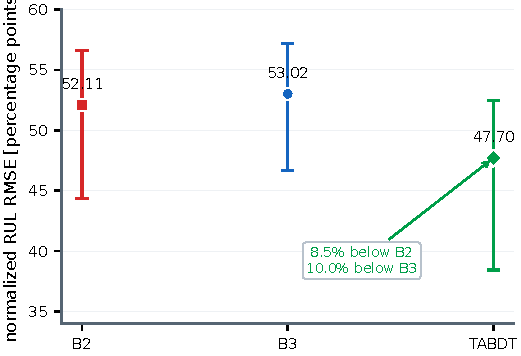
\includegraphics[width=0.95\columnwidth]{fig6_xjtu}
\caption{XJTU-SY age-compensation test at $p=0.02$. Bars are bearing-clustered
95\% intervals; network repetitions are not independent specimens.}
\label{fig:xjtu}
\end{figure}

\emph{6) Stress tests beyond the model assumptions:}
Figure~\ref{fig:stress} reports two tests on the same 400-unit population.
First, a two-state Markov link fixes the timely fraction at 0.05 while the
mean outage length increases from 20 to 80 steps. TABDT retains the observed
method ordering under these bursts, although the independent-delay
certificate does not cover this case~\cite{quevedo2013tac}; the result is
therefore empirical. Second, retrospective reprocessing of every received
measurement provides a reference posterior for assessing the forward
approximation. TABDT's RMSE exceeds this reference by 11.9\% at $p=0.02$,
0.9\% at $p=0.2$, and 0\% at $p=1$. Exact reprocessing requires
$O(tn^3+Stn^2)$ work per evaluation at time $t$ ($O(St)$ for fixed $n=2$),
whereas TABDT retains the online complexity reported above.

\begin{figure}[!t]
\centering
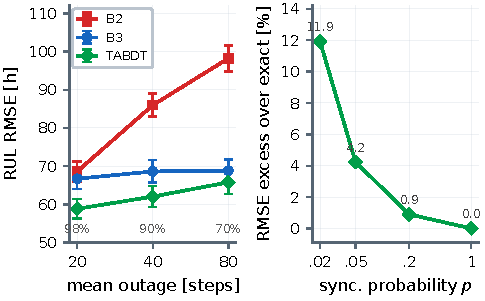
\includegraphics[width=\columnwidth]{fig8_stress}
\caption{Stress tests. Left: Markov-link RMSE at timely fraction 0.05
(descriptive bars as in Section~\ref{sec:metrics}; delivered fractions below).
Right: TABDT excess over exact replay on a common 25-step grid.}
\label{fig:stress}
\end{figure}

\emph{7) Network-aware maintenance decisions:}
Figure~\ref{fig:cost} translates the network-dependent certificate into the
maintenance surrogate \eqref{eq:cost}. Analytical curves are shown for three
network conditions and compared with separate Monte Carlo policy simulations
of 1\,500 known-drift, single-sensor anchor paths per point. For the sampled
points with $\xi\leq9.0$, the two cost rates
agree within 0.6\%. The approximation deteriorates near $D$, as expected
because the surrogate neglects diffusion overshoot: at
$(p,\xi)=(0.2,9.5)$, the simulated rate is 7.3\% higher. These sampled points
show that overshoot matters near $D$ but do not establish a general
safety-margin cutoff.

Within its stated conditions, the optimum moves earlier as the network
deteriorates. Specifically, $\xi^{*}$ is 9.42 at $p=0.9$, 9.34 at $p=0.5$,
and 9.18 at $p=0.2$. The corresponding safety margin widens from 0.58 to
0.82 HI, while the minimum surrogate cost increases from $2.135$ to
$2.197\times10^{-3}$ per hour. Both sufficient conditions in
Proposition~\ref{prop:threshold} hold at these operating points; the smallest
value of $(r^*)^2\xi^*$ is 88.5, compared with $D=10$.

\begin{figure}[!t]
\centering
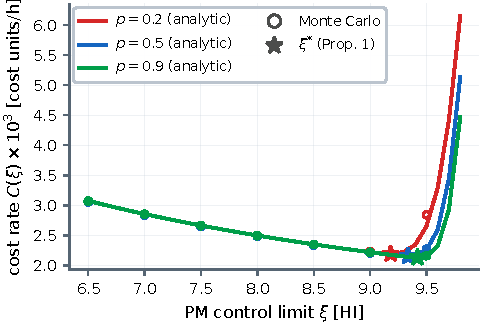
\includegraphics[width=\columnwidth]{fig7_cost}
\caption{Long-run cost rate against PM limit $\xi$: \eqref{eq:cost}, 1\,500-path
anchor simulations, and $\xi^*$. Under Proposition~\ref{prop:threshold}'s
conditions, poorer synchronization moves $\xi^*$ earlier.}
\label{fig:cost}
\end{figure}

\subsection{Threats to Validity and Limitations}
Three limitations delimit the claims made here. First,
Theorem~\ref{thm:bound} concerns a linear Gaussian, known-drift,
single-sensor, fresh-only anchor with independent packet arrivals. The
Markov-outage experiment examines correlated delivery only empirically
~\cite{quevedo2013tac}. Second, the main study is
synthetic and uses fixed trust scores. The XJTU-SY experiment evaluates the
packet-use rule on a single peak-amplitude proxy from 15 accelerated bearing
lives; it is not a full validation of the degradation model. Third, TABDT's
forward OOSM correction omits correlations retained by exact retrodiction
~\cite{barshalom2002,barshalom2004}. Its measured error relative to exact
reprocessing is empirical, and the maintenance expression \eqref{eq:cost}
remains a surrogate. The external interval coverage of 76.9\% reinforces
these limits. Nonlinear degradation, online trust estimation, correlated
fading, implementation profiling, and plant trials remain necessary before
deployment.

\section{Conclusion}\label{sec:conclusion}
TABDT combines age compensation and sensor-specific precision within a
Bayesian degradation twin, then uses a network-dependent variance certificate
to inform the preventive-maintenance limit. In a 4\,000-path anchor
experiment, the bound is within 1.3\% of empirical variance. In the separate
400-unit study, TABDT reduces RUL RMSE by as much as 27.9\%, and the nominal
intervals cover 93.4--95.6\% of observations.
Across 15 XJTU-SY bearing lives, normalized RMSE falls to 47.70 points from
52.11 and 53.02 for the two delayed-packet baselines. The corresponding
coverage of 76.9\% identifies interval calibration under measured degradation
as the principal requirement before plant deployment.

\begin{thebibliography}{22}

\bibitem{liu2024ticps}
R. Liu, Q. Zhang, T. Han, B. Yang, W. Zhang, S. Yin, and D. Zhou, ``Survey on
foundation models for prognostics and health management in industrial
cyber-physical systems,'' \emph{IEEE Trans. Ind. Cyber-Phys. Syst.}, vol. 2,
pp. 264--280, 2024, doi:
\href{https://doi.org/10.1109/TICPS.2024.3425326}{10.1109/TICPS.2024.3425326}.

\bibitem{zhang2024ticps}
J. Zhang, J. Tian, H. Luo, S. Wu, S. Yin, and O. Kaynak, ``Prognostics for
the sustainability of industrial cyber-physical systems: From an artificial
intelligence perspective,'' \emph{IEEE Trans. Ind. Cyber-Phys. Syst.}, vol. 2,
pp. 495--507, 2024, doi:
\href{https://doi.org/10.1109/TICPS.2024.3433492}{10.1109/TICPS.2024.3433492}.

\bibitem{tao2019}
F. Tao, H. Zhang, A. Liu, and A. Y. C. Nee, ``Digital twin in industry:
State-of-the-art,'' \emph{IEEE Trans. Ind. Informat.}, vol. 15, no. 4, pp.
2405--2415, Apr. 2019, doi:
\href{https://doi.org/10.1109/TII.2018.2873186}{10.1109/TII.2018.2873186}.

\bibitem{samanazari2024ticps}
M. S. Azari, L. Ricci, S. Santini, and F. Flammini, ``An intelligent
diagnostic framework based on digital twins and partial transfer learning:
Methodology and industrial application,'' \emph{IEEE Trans. Ind. Cyber-Phys.
Syst.}, vol. 3, pp. 1--13, 2025, doi:
\href{https://doi.org/10.1109/TICPS.2024.3490502}{10.1109/TICPS.2024.3490502}.

\bibitem{kumar2025ticps}
A. Kumar and N. Kumar, ``State-space driven digital twin for condition
monitoring and predictive health assessment in grid-integrated power converter
system,'' \emph{IEEE Trans. Ind. Cyber-Phys. Syst.}, vol. 3, pp. 464--471,
2025, doi:
\href{https://doi.org/10.1109/TICPS.2025.3586823}{10.1109/TICPS.2025.3586823}.

\bibitem{alkarawi2026dt}
Y. Al-Karawi, H. S. Mogheer, K. K. Hasan, and A. H. Dawwd, ``Digital twin
and native-AI empowered 6G networks: Architectures, applications, evaluation,
and open challenges,'' in \emph{Proc. Int. Russian Smart Industry Conf.
(SmartIndustryCon)}, 2026, pp. 13--20, doi:
\href{https://doi.org/10.1109/SmartIndustryCon68821.2026.11493034}{10.1109/SmartIndustryCon68821.2026.11493034}.

\bibitem{nist2023}
E. Tabassi, \emph{Artificial Intelligence Risk Management Framework (AI RMF
1.0)}, NIST AI 100-1, National Institute of Standards and Technology,
Gaithersburg, MD, USA, 2023, doi:
\href{https://doi.org/10.6028/NIST.AI.100-1}{10.6028/NIST.AI.100-1}.

\bibitem{ding2024tim}
Z.-Q. Ding, Q. Qin, Y.-F. Zhang, and Y.-H. Lin, ``An uncertainty
quantification and calibration framework for RUL prediction and accuracy
improvement,'' \emph{IEEE Trans. Instrum. Meas.}, vol. 73, Art. no. 2535613,
pp. 1--13, 2024, doi:
\href{https://doi.org/10.1109/TIM.2024.3485392}{10.1109/TIM.2024.3485392}.

\bibitem{sinopoli2004}
B. Sinopoli, L. Schenato, M. Franceschetti, K. Poolla, M. I. Jordan, and
S. S. Sastry, ``Kalman filtering with intermittent observations,''
\emph{IEEE Trans. Autom. Control}, vol. 49, no. 9, pp. 1453--1464, Sep.
2004, doi:
\href{https://doi.org/10.1109/TAC.2004.834121}{10.1109/TAC.2004.834121}.

\bibitem{yates2021}
R. D. Yates, Y. Sun, D. R. Brown, S. K. Kaul, E. Modiano, and S. Ulukus,
``Age of information: An introduction and survey,'' \emph{IEEE J. Sel.
Areas Commun.}, vol. 39, no. 5, pp. 1183--1210, May 2021, doi:
\href{https://doi.org/10.1109/JSAC.2021.3065072}{10.1109/JSAC.2021.3065072}.

\bibitem{ahmad2023jiot}
N. Ahmad, M. Egan, J.-M. Gorce, J. S. Dibangoye, and F. Le Mou\"el,
``Codesigned communication and data analytics for condition-based maintenance
in smart buildings,'' \emph{IEEE Internet Things J.}, vol. 10, no. 18, pp.
15847--15856, Sep. 2023, doi:
\href{https://doi.org/10.1109/JIOT.2023.3266029}{10.1109/JIOT.2023.3266029}.

\bibitem{yang2022jiot}
T. Yang and C. Lv, ``A secure sensor fusion framework for connected and
automated vehicles under sensor attacks,'' \emph{IEEE Internet Things J.},
vol. 9, no. 22, pp. 22357--22365, Nov. 2022, doi:
\href{https://doi.org/10.1109/JIOT.2021.3101502}{10.1109/JIOT.2021.3101502}.

\bibitem{feng2023ticps}
K. Feng, Y. Xu, Y. Wang, S. Li, Q. Jiang, B. Sun, J. Zheng, and Q. Ni,
``Digital twin enabled domain adversarial graph networks for bearing fault
diagnosis,'' \emph{IEEE Trans. Ind. Cyber-Phys. Syst.}, vol. 1, pp. 113--122,
2023, doi:
\href{https://doi.org/10.1109/TICPS.2023.3298879}{10.1109/TICPS.2023.3298879}.

\bibitem{si2014}
X.-S. Si, W. Wang, C.-H. Hu, and D.-H. Zhou, ``Estimating remaining useful
life with three-source variability in degradation modeling,'' \emph{IEEE
Trans. Rel.}, vol. 63, no. 1, pp. 167--190, Mar. 2014, doi:
\href{https://doi.org/10.1109/TR.2014.2299151}{10.1109/TR.2014.2299151}.

\bibitem{huang2015}
Z. Huang, Z. Xu, W. Wang, and Y. Sun, ``Remaining useful life prediction for
a nonlinear heterogeneous Wiener process model with an adaptive drift,''
\emph{IEEE Trans. Rel.}, vol. 64, no. 2, pp. 687--700, Jun. 2015, doi:
\href{https://doi.org/10.1109/TR.2015.2403433}{10.1109/TR.2015.2403433}.

\bibitem{zhai2017}
Q. Zhai and Z.-S. Ye, ``RUL prediction of deteriorating products using an
adaptive Wiener process model,'' \emph{IEEE Trans. Ind. Informat.}, vol.
13, no. 6, pp. 2911--2921, Dec. 2017, doi:
\href{https://doi.org/10.1109/TII.2017.2684821}{10.1109/TII.2017.2684821}.

\bibitem{barshalom2002}
Y. Bar-Shalom, ``Update with out-of-sequence measurements in tracking:
Exact solution,'' \emph{IEEE Trans. Aerosp. Electron. Syst.}, vol. 38, no.
3, pp. 769--777, Jul. 2002, doi:
\href{https://doi.org/10.1109/TAES.2002.1039398}{10.1109/TAES.2002.1039398}.

\bibitem{barshalom2004}
Y. Bar-Shalom, H. Chen, and M. Mallick, ``One-step solution for the multistep
out-of-sequence-measurement problem in tracking,'' \emph{IEEE Trans. Aerosp.
Electron. Syst.}, vol. 40, no. 1, pp. 27--37, Jan. 2004, doi:
\href{https://doi.org/10.1109/TAES.2004.1292140}{10.1109/TAES.2004.1292140}.

\bibitem{greiff2024cdc}
M. Greiff and K. Berntorp, ``Asynchronous variational-Bayes Kalman
filtering,'' in \emph{Proc. 63rd IEEE Conf. Decision Control (CDC)}, Milan,
Italy, 2024, pp. 1987--1992, doi:
\href{https://doi.org/10.1109/CDC56724.2024.10886035}{10.1109/CDC56724.2024.10886035}.

\bibitem{quevedo2013tac}
D. E. Quevedo, A. Ahl\'en, and K. H. Johansson, ``State estimation over
sensor networks with correlated wireless fading channels,'' \emph{IEEE
Trans. Autom. Control}, vol. 58, no. 3, pp. 581--593, Mar. 2013, doi:
\href{https://doi.org/10.1109/TAC.2012.2212515}{10.1109/TAC.2012.2212515}.

\bibitem{yang2024tr}
L. Yang, Y. Chen, X. Ma, Q. Qiu, and R. Peng, ``A prognosis-centered
intelligent maintenance optimization framework under uncertain failure
threshold,'' \emph{IEEE Trans. Rel.}, vol. 73, no. 1, pp. 115--130, Mar.
2024, doi:
\href{https://doi.org/10.1109/TR.2023.3273082}{10.1109/TR.2023.3273082}.

\bibitem{wang2020xjtu}
B. Wang, Y. Lei, N. Li, and N. Li, ``A hybrid prognostics approach for
estimating remaining useful life of rolling element bearings,''
\emph{IEEE Trans. Rel.}, vol. 69, no. 1, pp. 401--412, Mar. 2020, doi:
\href{https://doi.org/10.1109/TR.2018.2882682}{10.1109/TR.2018.2882682}.

\end{thebibliography}

\end{document}
